\documentclass{beamer}
%Information to be included in the title page:
\title{Do cryptocurrencies extend the mean-variance frontier of an equity investor?}
\author{Sander Naerum, Thomas Pietsch and Ziga Jagodnik}
\institute{UZH}
\date{2023}

\begin{document}

\frame{\titlepage}

\begin{frame}
\frametitle{The Project}
In this project we will investigate if cryptocurrencies extend the mean-variance frontier of an equity investor. 
By using an industry portfolio dataset consisting of 12 different industries collected from Kenneth French data 
library combined with the 3 largest cryptocurrencies based on market capitalization, we extract the mean-variance 
frontier. We show that adding cryptocurrencies to the mean-variance frontier has a significant impact.
\end{frame}

\begin{frame}
\frametitle{Data}
\textbf{Equity data:} Kenneth French website, 12 industry portfolios. The assets within the industry portfolios are 
equally weighted and the data downloaded has daily frequency. 

\noindent\textbf{Crypto's:} Imported the 3 largest crypto currencies based on market cap, source: Yahoo Finance. 
Can also be extended in the data grabbing. Crypto data is downloaded with daily frequency.  

\noindent \textbf{Caveat:} We only have data from 2017-2023 on the cryptocurrencies. Ideally, to conclude that 
cryptocurrencies actually extends the mean-variance frontier of an equity investor, we would want data on a longer time frame.    
\end{frame}


\begin{frame}
\frametitle{Analysis}
\begin{figure}
    \centering
    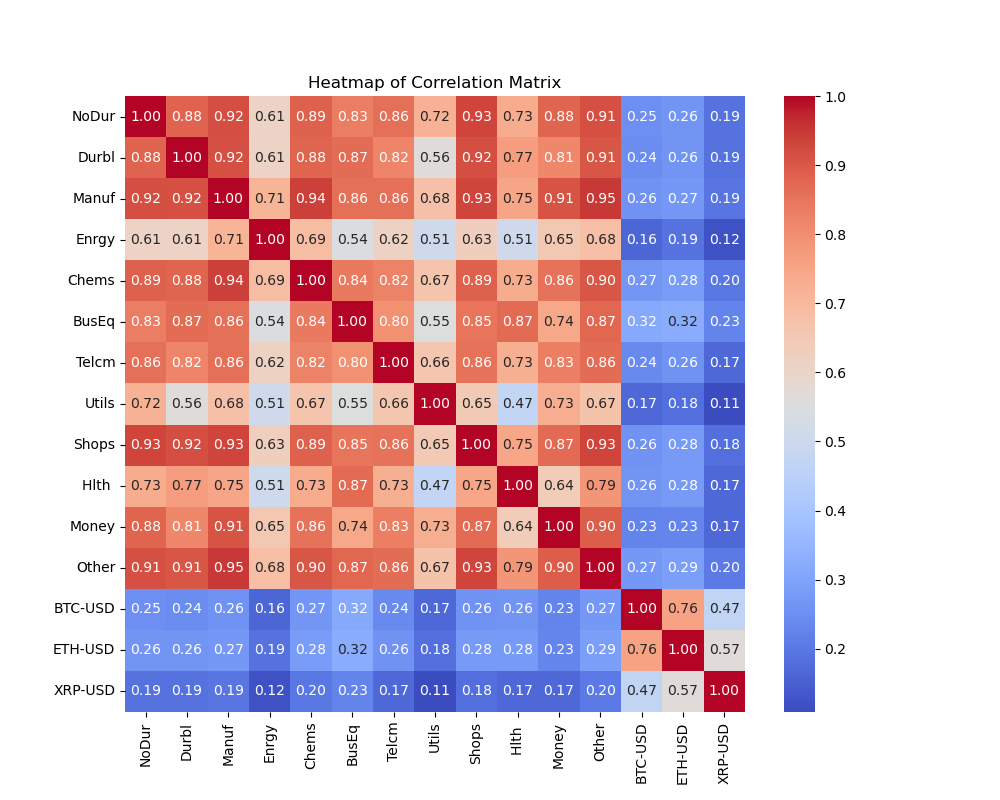
\includegraphics[width=0.8\linewidth]{Figures/heatmap_correlation.png}
    \caption{Full sample correlations}
    \label{fig:corr}
\end{figure}
\end{frame}

\begin{frame}
\frametitle{Analysis}
\begin{figure}
    \centering
    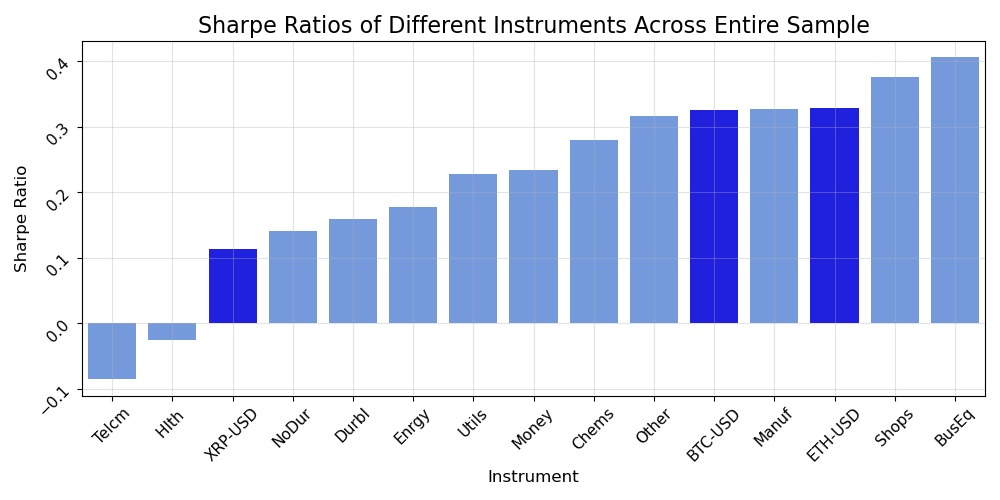
\includegraphics[width=0.8\linewidth]{Figures/SR_Entire_Sample.png}
    \caption{Full sample Sharpe's}
    \label{fig:sharpe}
\end{figure}
\end{frame}

\begin{frame}
\frametitle{Results}
\begin{figure}
    \centering
    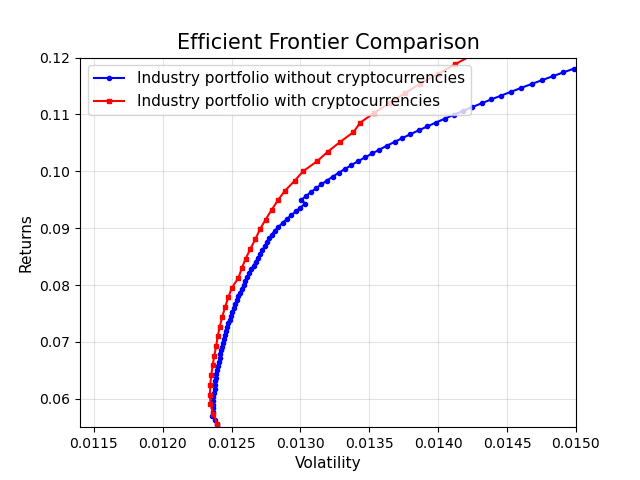
\includegraphics[width=0.8\linewidth]{Figures/Efficient_Frontier_Comparison_Full_Sample.png}
    \caption{Full sample}
    \label{fig:full}
\end{figure}
\end{frame}

\begin{frame}
\frametitle{Results}
\begin{figure}
    \centering
    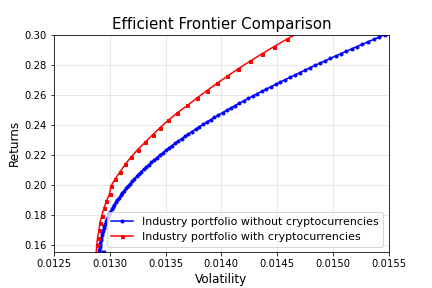
\includegraphics[width=0.8\linewidth]{Figures/Efficient_Frontier_Comparison_Bull_Market.png}
    \caption{Restricted sample}
    \label{fig:restricted}
\end{figure}
\end{frame}

\begin{frame}
\frametitle{Conclusion}
The inclusion of cryptocurrencies in an investment portfolio extends the mean-variance frontier for an equity investor, 
introducing a new dimension to diversification strategies and expanding the spectrum of risk and return possibilities.
 \nocite{wikiref}
\end{frame}

\begin{frame}
\frametitle{Bibliography}

\bibliographystyle{apalike}
\bibliography{References}
\end{frame}

\end{document}